\chapter{Metodolog\'ia.}

\section{Elaboraci\'on de la base de datos.}


\hspace{0.4cm} La fuente principal de informaci\'on para calcular la curva de rendimientos para los t\'itulos de la deuda p\'ublica nacional es el Banco Central de Venezuela (BCV), el cual diariamente publica las operaciones realizadas con dichos instrumentos y los muestra en el documento ``resumersec"\hspace{0.01cm} en la pesta\~na $``0-22"$ (Ver Figura 1), en el mismo se puede encontrar la informaci\'on sobre el c\'odigo del instrumento, su fecha de vencimiento, su plazo, la cantidad de operaciones, el monto en Bol\'ivares, el precio m\'inimo, m\'aximo y promedio, y el cup\'on asociado a cada instrumento.

\vspace{0.5cm}

\begin{figure}[h]
  \scalebox{0.50}{\includegraphics{images/Imagen022.png}}
%\includegraphics[width=0.7\textwidth]{Imagen022.png}
\caption{Pesta\~na ``0-22".}
\end{figure}

\vspace{0.5cm}

\hspace{0.4cm} Es importante recordar que dentro de los t\'itulos de la Deuda P\'ublica Nacional se encuentran los t\'itulos de inter\'es fijo (TIF) y los t\'itulos de tasa variable (VEBONO), los primeros se caracterizan por poseer una tasa de cup\'on que no varia, por su parte los VEBONO poseen una tasa de inter\'es variable.

\vspace{0.5cm}

\hspace{0.4cm}Esta informaci\'on tambi\'en es suministrada por el BCV, en su documento de las ``Caracter\'isticas de la Deuda P\'ublica Nacional" (Ver Figura 2), por lo cual el mismo se debe revisar con cierta frecuencia, con el fin de actualizar la tasa de cup\'on de los VEBONO.


\begin{figure}[h]
  \scalebox{0.50}{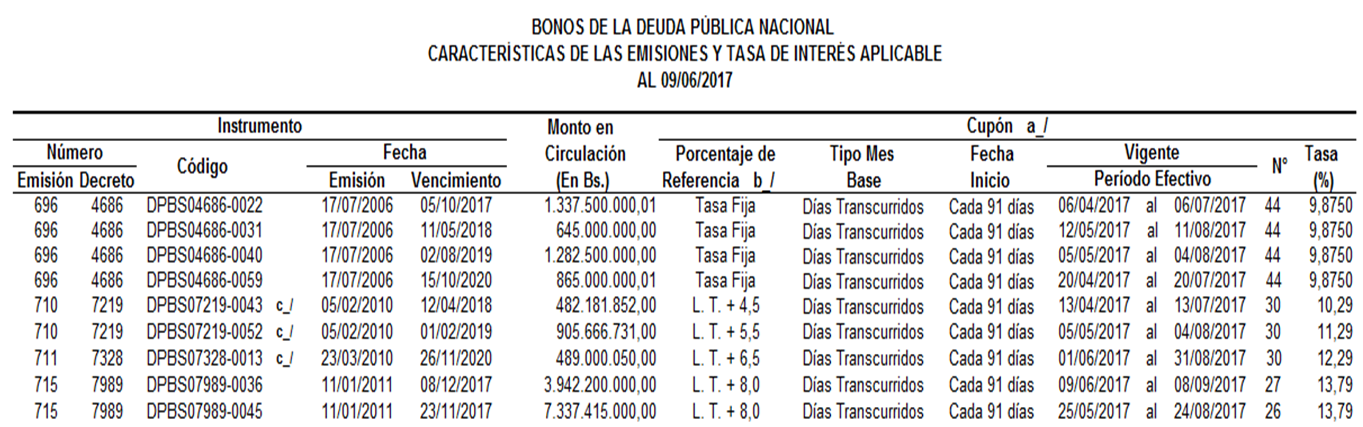
\includegraphics{images/Imagencarac.png}}
\caption{Caracter\'isticas.}
\end{figure}


\hspace{0.4cm} A partir de la pesta\~na ``0-22"\hspace{0.01cm} y del documento de las caracter\'isticas, se cre\'o la base de datos con la cual se va a trabajar, la misma contiene no s\'olo la informaci\'on suministrada por la pesta\~na ``0-22", sino alguna informaci\'on adicional tomada del documento de las caracter\'isticas. En dicha base de datos se contar\'a con la siguiente informaci\'on,

\vspace{0.5cm}

\begin{itemize}
  \item Tipo Instrumento: Indica el tipo de instrumento.
  \item Nombre: Proporciona el nombre corto del t\'itulo, usualmente este nombre se conforma por el tipo de t\'itulo m\'as su mes y a\~no de vencimiento, por ejemplo, el t\'itulo TIF032028, representa al t\'itulo TIF con vencimiento en marzo del 2028.
  \item Fecha de operaci\'on: Indica la fecha en que se efectu\'o dicha operaci\'on.
  \item Fuente: Indica la fuente de donde se tom\'o la informaci\'on, esta se puede tomar de dos fuentes, la primera mediante la pesta\~na 0-22 (mercado secundario) y  la otra mediante el documento de las subastas (mercado primario, informaci\'on suministrada por el BCV).
  \item Sicet: Proporciona el c\'odigo asociado a cada t\'itulo.
  \item Fecha de vencimiento: Indica la fecha de maduraci\'on (vencimiento) del instrumento.
  \item Plazo: Indica la cantidad de d\'ias que falta para que el instrumento se venza.
  \item Cantidad de operaciones: Proporciona la cantidad de operaciones efectuadas con un insrumento en espec\'ifico.
  \item Monto: Indica el monto en Bol\'ivares, por el cual se efectu\'o la operaci\'on u operaciones.
  \item Precio m\'inimo: Indica el precio m\'inimo, por el cual se trans\'o la operaci\'on.
  \item Precio m\'aximo: Indica el precio m\'aximo, por el cual se trans\'o la operaci\'on.
  \item Precio promedio: Indica el precio promedio, por el cual se trans\'o la operaci\'on, cabe destacar que en dado caso de existir una sola operaci\'on el valor del precio m\'inimo, m\'aximo y promedio van a coincidir.
  \item Cup\'on: Proporciona la tasa de cup\'on asociado a cada instrumento.
  \item Frecuencia: Indica con que frecuencia el instrumento paga cup\'on, para los TIF y VEBONO, esta es 4, pues los mismos pagan cu\'pon trimestralmente, as\'i se obtiene este valor pues existen 4 trimestres en el a\~no.

\end{itemize}

\vspace{0.5cm}

\hspace{0.4cm} Una vez obtenida la base de datos esta seg\'un sea el caso puede ser depurada mediante ciertos criterios, el primero es que aquellas operaciones con un monto menor a los 10 milllones no se consideran. El segundo es el tipo de fuente, siempre prevalecer\'a la fuente subasta. El tercero es considerar la operaci\'on mas reciente, es decir, si en la base de datos se tiene que para un mismo instrumento existen diferentes operaciones en diferentes d\'ias, s\'olo se considerar\'a la operaci\'on m\'as reciente.

\vspace{0.5cm}

\hspace{0.4cm} Para efectuar la depuraci\'on, a la base de datos anterior se le a\~nadir\'an dos columnas nuevas una que indica el rendimiento al vencimiento de cada instrumento y la otra que indica la decisi\'on que se tom\'o en base a los criterios descritos anteriormente (Ver Figura 3). Esta \'ultima ser\'a una variable dicot\'omica, es decir solo con dos valores (0 \'o 1), en donde ``0" me indica que no selecciono el t\'itulo y ``1" me indica que si lo tomo en cuenta para el estudio a realizar.\\

\begin{figure}[h]
  \scalebox{0.50}{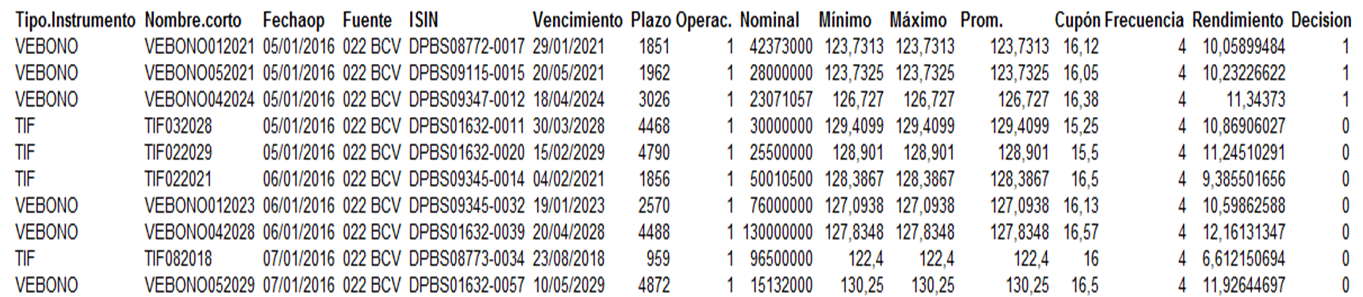
\includegraphics{images/Imagenbase.png}}
\caption{Base de datos.}
\end{figure}


\section{Estimaci\'on de par\'ametros y curva de rendimiento.}

\hspace{0.4cm} Una vez construida la base de datos, se proceder\'a a utilizar los splines de suavizado para obtener los par\'ametros necesarios para la curva de rendimientos. Recordemos que esta curva relaciona el plazo del instrumento con su rendimiento.

\vspace{0.5cm}

\hspace{0.4cm} Es importante se\~nalar que se estimar\'a una curva por cada tipo de instrumento, as\'i se obtendr\'a un curva para los TIF y una curva para los VEBONO. Por tal raz\'on a partir de la base de datos, se separar\'a los TIF de los VEBONOS, y se considerar\'an s\'olo las columnas Plazo y Rendimiento para estimar dicha curva. Seg\'un sea el caso, s\'olo considerar\'an aquellas observaciones que tengan decisi\'on 1.


\hspace{0.4cm} Aunado a cada tipo de instrumento (TIF \'o VEBONO), se considerar\'a un instrumento de otro tipo este es la letra del tesoro, este tipo de instrumento representar\'a el punto inicial la curva, cabe destacar que la letra a considerar debe ser aquella cuya fecha de operaci\'on sea la m\'as reciente con respecto a la fecha de valoraci\'on (d\'ia en que se quiere conocer los rendimientos estimados).

\vspace{0.5cm}

\hspace{0.4cm} A partir de la curva de rendimientos obtenida (Ver Figura 4) es posible calcular un rendimiento estimado para alg\'un tipo de instrumento a partir de su plazo, que no es m\'as que la cantidad de d\'ias que faltan por transcurrir hasta su vencimiento. Este valor es de suma importancia ya que a partir del mismo es posible calcular el precio estimado asociado a cada instrumento en un d\'ia espec\'ifico. Con lo cual es posible saber a partir de la historia (base de datos), el precio estimado de alg\'un instrumento que le interese a cierta instituci\'on y por ende saber si ese t\'itulo es rentable o no, es decir, si vale la pena invertir en el mismo o no.\\

\begin{figure}[h]
  \scalebox{0.40}{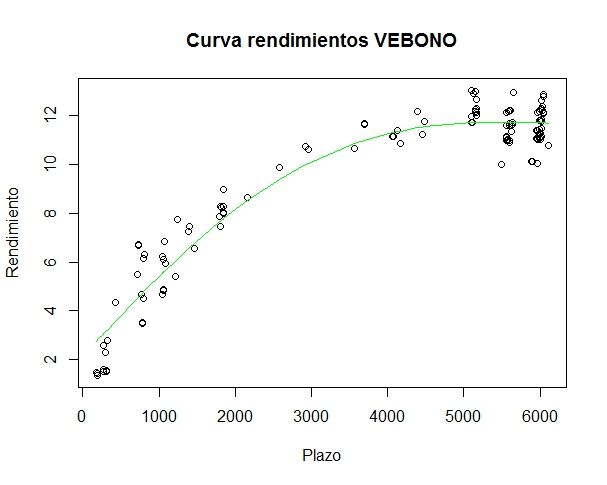
\includegraphics{images/curvarend.jpeg}}
\caption{Curva de Rendimiento.}
\end{figure}



